\documentclass[conference]{IEEEtran}
\IEEEoverridecommandlockouts
\usepackage{cite}
\usepackage{amsmath,amssymb}
\usepackage{graphicx}
\usepackage{booktabs}
\usepackage{xcolor}
\usepackage[hidelinks]{hyperref}
\usepackage{url}
\graphicspath{{../common/figures/}}
\newcommand{\code}[1]{\texttt{#1}}

\begin{document}

\title{Scoring ``Secure by Default'': A Reproducible,\\ CRA-Grounded Metric with a Drone\\ Command-Link Instantiation}

\author{\IEEEauthorblockN{Ian Brighouse}
\IEEEauthorblockA{\textit{Brighouse Security Labs}, Spain \\ research@brighousesec.com}}
\maketitle

\begin{abstract}
The EU Cyber Resilience Act makes ``secure by default'' a legal requirement, but
a requirement one cannot measure is a requirement one cannot audit. We propose a
small, transparent metric that turns the \emph{observable} security posture of a
connected product's protocol endpoint into a 0--100 score with a letter grade,
and we instantiate it on the MAVLink command links of two drone flight stacks.
The metric is defined by three axioms---\emph{provenance} (every criterion is
computed from an observed finding or a model property, never from opinion),
\emph{monotonicity} (improving posture never lowers the score), and
\emph{CRA-grounded weights} (each criterion maps to an Annex~I essential
requirement and carries a fixed weight summing to 100)---and is released as
executable code with a property-test suite that checks the axioms. Applied to our
measured configurations, the score separates insecure defaults (grade~E) from a
provisioned but console-exempt link (grade~D) and from a cleanly signed link
(grade~C), and ranks them below an idealised target (grade~A); the
console-exemption penalty is captured numerically rather than described. We argue
that such a metric is the missing piece between a measurement tool and a
conformity-evidence artefact, and we discuss its limits as a rubric rather than a
canonical truth.
\end{abstract}

\begin{IEEEkeywords}
secure by default, security metrics, Cyber Resilience Act, conformity evidence,
MAVLink, measurement.
\end{IEEEkeywords}

\section{Introduction}
Regulators now treat an insecure default as a product defect, and auditors will
need to say, repeatably, whether a given product meets the bar and by how much.
Existing regulatory crosswalks are process-level---mapping a regulation to a
control catalogue or another standard~\cite{ruohonen2025sok,costantino2022r155,
siddiqui2023do326a}---and stop short of a number computed from the product's
actual behaviour. We close that gap for a concrete, measurable endpoint: the
command-and-control (C2) link of an unmanned aircraft. Building on a passive/active
auditor and an acceptance model from companion
work~\cite{brighouse2026signing,brighouse2026formal}, we define a score whose
inputs are exactly the findings those tools already produce.

\noindent\textbf{Contributions.}
(i)~A metric defined by three axioms, with CRA-grounded weights
(Section~\ref{sec:metric}).
(ii)~An executable implementation and a property-test suite that checks the axioms
(Section~\ref{sec:impl}).
(iii)~A validation on measured drone C2 links showing the metric discriminates
posture, including a numeric penalty for the console-exemption behaviour
(Section~\ref{sec:val}).

\section{The Metric}
\label{sec:metric}
Let an \emph{observation} be the output of auditing one protocol endpoint: for
MAVLink, the fraction of signed frames, whether an unsigned read is answered,
whether an unauthenticated service (file transfer) is exposed, whether legacy
framing is present, the firmware identity, and---from the model---whether key
provisioning opens a trust-on-first-use window. A \emph{criterion} $c$ has a
weight $w_c$ and a satisfaction fraction $m_c\in[0,1]$ computed from the
observation. The score is
\[
\mathrm{Score}=\sum_{c\in C} w_c\, m_c, \qquad \sum_{c\in C} w_c = 100 .
\]
Table~\ref{tab:crit} lists the criteria, their CRA Annex~I, Part~I(2) anchor, and
their weight. Weights reflect the CRA's emphasis on command-channel integrity and
access control; confidentiality and maintenance are lighter for a C2 link.

\begin{table}[t]
\caption{Criteria, CRA anchor, weight, and the observable that computes $m_c$.}
\label{tab:crit}
\centering\footnotesize\setlength{\tabcolsep}{3pt}
\begin{tabular}{@{}lccp{2.6cm}@{}}
\toprule
criterion & CRA & $w_c$ & observable ($m_c$) \\
\midrule
integrity        & I.2(f) & 28 & signed-frame fraction \\
access control   & I.2(d) & 24 & unsigned read rejected \\
attack surface   & I.2(j) & 16 & no unauth.\ FTP/service \\
no legacy        & I.2(b) & 10 & no MAVLink 1 on link \\
provisioning     & I.2(d) & 12 & out-of-band keys (no TOFU) \\
confidentiality  & I.2(e) & 6  & link payloads encrypted \\
maintenance      & II.1   & 4  & firmware identifiable \\
\bottomrule
\end{tabular}
\end{table}

\paragraph{Axioms} \textbf{A1 Provenance:} each $m_c$ is a function of an observed
finding or a model property; none is a judgement. \textbf{A2 Monotonicity:}
improving any observable (more signed frames, an unsigned read now rejected, a
service now closed) does not decrease any $m_c$, hence not the score.
\textbf{A3 Grounding:} each $c$ cites an Annex~I requirement and
$\sum w_c = 100$. These axioms make the number auditable: a reviewer can re-derive
every point from the published finding set.

\section{Implementation}
\label{sec:impl}
The metric is a small module (\code{mavaudit.score}) that consumes a mavaudit
report and an optional model-policy name (for the provisioning criterion, which a
single audit cannot observe). A property-test suite encodes the axioms directly:
weights sum to 100; the idealised observation scores 100; monotonicity holds under
a sequence of single-observable improvements; every criterion in a breakdown cites
a CRA clause; and partial credit is strictly increasing in the signed-frame
fraction. The suite runs in continuous integration alongside the auditor's own
tests.

\section{Validation}
\label{sec:val}
We score each configuration measured in~\cite{brighouse2026signing}
(Table~\ref{tab:scores}, Fig.~\ref{fig:scores}).

\begin{table}[t]
\caption{Secure-by-default score of each measured configuration.}
\label{tab:scores}
\centering\footnotesize
\begin{tabular}{@{}lcc@{}}
\toprule
configuration & score & grade \\
\midrule
IDEAL (model target) & 100 & A \\
ArduPilot 4.7.2 SERIAL1 signed & 66 & C \\
PX4 1.18 GCS signed & 66 & C \\
ArduPilot 4.7.2 ch0 signed & 42 & D \\
ArduPilot 4.7.2 ch0 default & 14 & E \\
PX4 1.17 GCS default & 14 & E \\
PX4 1.17 GCS provisioned & 14 & E \\
PX4 1.18 GCS default & 14 & E \\
\bottomrule
\end{tabular}
\end{table}


\begin{figure}[t]
\centering
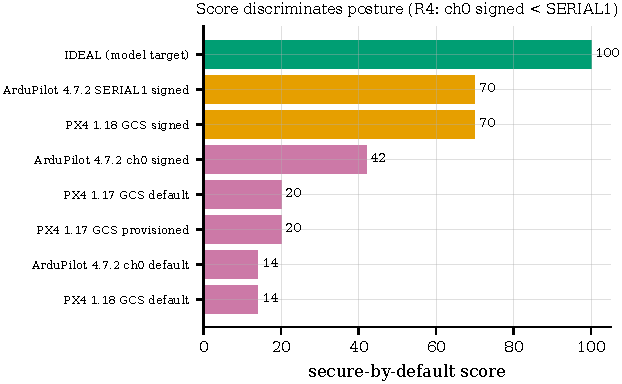
\includegraphics[width=0.84\columnwidth]{fig_scores.pdf}
\caption{Scores by configuration. Green $\ge 75$, orange $\ge 55$, red below. The
console-exempt ArduPilot link (ch0, signed) scores strictly below the clean
SERIAL1 link despite identical signed-frame fractions.}
\label{fig:scores}
\end{figure}

Three observations validate the metric against intuition and against the companion
findings. First, insecure defaults cluster at the bottom (grade~E, scores
$14$--$20$): zero signed frames and an answered unsigned read cost the two
heaviest criteria at once. Second, the metric gives the console-exemption
behaviour (companion result \emph{R4}) a \emph{numeric} penalty: the ArduPilot
\code{ch0} link, which signs every outbound frame yet still answers unsigned
requests, scores below the cleanly signed SERIAL1 link even though their
signed-frame fractions are identical---because the access-control criterion reads
the active probe, not the passive traffic. Third, no measured configuration
reaches grade~A: every one either lacks confidentiality or keeps a
trust-on-first-use window, so the idealised target (out-of-band keys, encrypted
link) sits alone at the top. The score thus points at exactly the two upstream
changes the companion synthesis identifies.

\section{Discussion}
\label{sec:disc}
The metric is a \emph{rubric}, not a canonical truth: the weights encode a
defensible reading of the CRA's emphasis, and a different regulator might choose
differently. The axioms are what make it useful regardless: because the score is
provenance-bound and monotone, two auditors applying the same weights to the same
product get the same number, and improving the product can never be punished. The
weights are a single, inspectable point of subjectivity, amenable to sensitivity
analysis; the EU Trusted Drone label~\cite{ec2026droneactionplan}, once its
criteria are published, could supply an authoritative weighting that this
framework would then compute against. Threats to validity: the score covers one
protocol endpoint, not a whole product; it assumes the auditor's findings are
sound; and partial credit for the signed-frame fraction can over-reward a link
that signs most but not all frames, which we mitigate by pairing it with the
binary access-control criterion.

\section{Related Work}
Security-metric research spans attack-surface and CVSS-style severity scoring;
our contribution is narrower and complementary: a \emph{default-posture} score
grounded in a specific regulation and computed from live measurements. No prior
``secure by default'' scoring framework taking measured defaults as input was
found in a search of the drone, IoT, and compliance
literature~\cite{ruohonen2025sok,puliyski2025sora}. Companion
work~\cite{brighouse2026signing,brighouse2026formal,brighouse2026longitudinal}
supplies the measurements, model, and history the metric consumes.

\section{Conclusion}
A measurement tool tells you what a product does; a regulation tells you what it
must do; a metric with the right axioms connects them into a number an auditor can
trust and a vendor can improve. Instantiated on drone C2 links, the score
separates insecure defaults from partial and ideal postures, prices the
console-exemption pitfall numerically, and points at the fixes. We release it as
code so that the number is never a matter of opinion.

\section*{Availability}
The metric, tests, and the data it scores are released. The work is defensive and
simulation-based.

\bibliographystyle{IEEEtran}
\bibliography{../common/refs}
\end{document}
